\documentclass[14pt,a4paper,report]{report}
\usepackage[a4paper, mag=1000, left=2.5cm, right=1cm, top=2cm, bottom=2cm, headsep=0.7cm, footskip=1cm]{geometry}
\usepackage[utf8]{inputenc}
\usepackage[english,russian]{babel}
\usepackage{indentfirst}
\usepackage[dvipsnames]{xcolor}
\usepackage[colorlinks]{hyperref}
\usepackage{listings} 
\usepackage{fancyhdr}
\usepackage{caption}
\usepackage{graphicx}
\hypersetup{
	colorlinks = true,
	linkcolor  = black
}

\usepackage{titlesec}
\titleformat{\chapter}
{\Large\bfseries} % format
{}                % label
{0pt}             % sep
{\huge}           % before-code


\DeclareCaptionFont{white}{\color{white}} 

% Listing description
\usepackage{listings} 
\DeclareCaptionFormat{listing}{\colorbox{gray}{\parbox{\textwidth}{#1#2#3}}}
\captionsetup[lstlisting]{format=listing,labelfont=white,textfont=white}
\lstset{ 
	% Listing settings
	inputencoding = utf8,			
	extendedchars = \true, 
	keepspaces = true, 			  	 % Поддержка кириллицы и пробелов в комментариях
	language = bash,            	 	 % Язык программирования (для подсветки)
	basicstyle = \small\sffamily, 	 % Размер и начертание шрифта для подсветки кода
	numbers = left,               	 % Где поставить нумерацию строк (слева\справа)
	numberstyle = \tiny,          	 % Размер шрифта для номеров строк
	stepnumber = 1,               	 % Размер шага между двумя номерами строк
	numbersep = 5pt,              	 % Как далеко отстоят номера строк от подсвечиваемого кода
	backgroundcolor = \color{white}, % Цвет фона подсветки - используем \usepackage{color}
	showspaces = false,           	 % Показывать или нет пробелы специальными отступами
	showstringspaces = false,    	 % Показывать или нет пробелы в строках
	showtabs = false,           	 % Показывать или нет табуляцию в строках
	frame = single,              	 % Рисовать рамку вокруг кода
	tabsize = 2,                  	 % Размер табуляции по умолчанию равен 2 пробелам
	captionpos = t,             	 % Позиция заголовка вверху [t] или внизу [b] 
	breaklines = true,           	 % Автоматически переносить строки (да\нет)
	breakatwhitespace = false,   	 % Переносить строки только если есть пробел
	escapeinside = {\%*}{*)}      	 % Если нужно добавить комментарии в коде
}

\begin{document}

\def\contentsname{Содержание}

% Titlepage
\begin{titlepage}
	\begin{center}
		\textsc{\largeСанкт-Петербургский Политехнический Университет Петра Великого\\[5mm]
Институт компьютерных наук и технологий\\[5mm]
Кафедра компьютерных систем и программных технологий\\[5mm]}
		
		\vfill
		
		\textbf{\LargeОтчет по лабораторному практикуму\\[3mm]
			\largeДисциплина: Аппаратные платформы встраиваемых систем\\[15mm]
		}
	\end{center}
	
	\vfill
\begin{flushright}
	\begin{minipage}{.4\textwidth}
		{\normalsizeВыполнили студенты гр.13541/1:\\[2mm] 
		\underline{\hspace{2in}}\\ % линия подчёркивания на два дюйма
  		\centering
  		\small(подпись)
		%Никитин А.Е.\\[5mm]
		Егоров Д.Е.\\[5mm]
		
		\underline{\hspace{2in}}\\ % линия подчёркивания на два дюйма
  		\centering
 		 \small(подпись)
		%Баринов М.С.\\[5mm]
		Чупин Н.С. \\[5mm]
				
		\normalsizeРуководитель:\\[2mm] 
		\underline{\hspace{2in}}\\ % линия подчёркивания на два дюйма
  		\centering
 		 \small(подпись)
		Васильев А.Е.\\
		}
	\end{minipage}
\end{flushright}
	\vfill
	\begin{center}
		Санкт-Петербург\\ \the\year\ г.
	\end{center}
\end{titlepage}

% Contents
\tableofcontents
\clearpage

\chapter {Лабораторная работа №1 «IAR, CMSIS, SPL, GPIO»}

\section {Цель работы}

Ознакомиться с интегрированной средой разработки IAR Embedded Workbench for ARM, а также функциями CMSIS и MDRSPL, получить навыки создания и отладки программного обеспечения для целевой платформы на примере разработки программ, взаимодействующих с портами ввода-вывода.

\section{Программа работы}

\begin{enumerate}
	\item Создать проект-заготовку для последующих лабораторных работ. Листинг демонстрационной программы приведен ниже.
	\item Подключить к проекту библиотеку CMSIS. Объяснить назначение и содержание файлов библиотеки. Объяснить назначение и содержание файла startup\_MDR32F9Qx.c
	\item Подключить к проекту библиотеку MDR32F9Qx Standart Peripherals Library.
	\item Настроить параметры отладчика для запуска демонстрационного примера на отладочной плате. Собрать проект, продемонстрировать его исполнение «по шагам».
	\item Разработать программу, включающую светодиоды на плате при нажатии кнопок; алгоритм согласовать с руководителем.
\end{enumerate}

Код демонстрационного примера приведен в листинге 1.1.

\lstinputlisting[caption=Код демонстрационного примера,language=c]{main1_1.c}

\section{Алгоритм переключения светодиодов}

По нажатию кнопки SELECT, двухразрядное двоичное число, отображаемое светодиодами должно инкреметироваться. 

Конечный автомат состояний программы представлен на рисунке 1.1, где st0 – состояние ожидания прерывания, а при переходе в состояние st1 вызывается подпрограмма обработки этого прерывания.

\begin{figure}[h!]
	\centering
	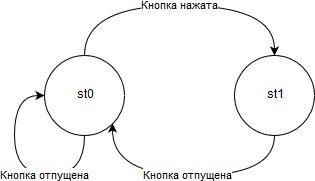
\includegraphics[scale = 1]{img/1_1.png}
	\caption{Схема конечного автомата программы}
\end{figure}

\section{Ход работы}

После настройки среды разработки IAR Embedded Workbench for ARM для работы с микросхемой Milandr, подключения необходимых библиотек и запуска демонстрационного проекта, код программы был запущен и протестирован на работоспособность. Затем были внесены изменения в соответствии с заданием преподавателя. Для этого был разработан конечный автомат, схема которого приведена выше. 
Код программы, разработанной в соответствии с индивидуальным заданием руководителя приведен в листинге 1.2. 

\lstinputlisting[caption=Код демонстрационного примера,language=c]{main1_2.c}


\section{Выводы}
По итогам лабораторной работы было произведено ознакомление с интегрированной средой разработки IAR Embedded Workbench for ARM, а также функциями CMSIS и MDRSPL. Также были получены навыки создания и отладки программного обеспечения для целевой платформы на примере разработки программ, взаимодействующих с портами ввода-вывода. \\
\indent Была реализована система управления миганием светодиодов. Отличительной чертой данной реализации является конечный автомат который обрабатывает нажатие кнопки, и при помощи программно реализованного триггера переключает состояния системы, сравнивая текущее её состояние с сохраненным предыдущим. \\
\indent Улучшение данной системы возможно путем использования обработчика прерываний. Это позволит оптимизировать работу системы, ввиду отсутствия лишней проверки на нажатие кнопки во время её работы.

\clearpage

\chapter {Лабораторная работа №2 «Системы тайминга и прерываний»}

\section {Цель работы}

Развитие навыков разработки встраиваемых приложений реального времени. 

\section{Программа работы}

\begin{enumerate}
	\item Изучит листинг программы, приведенной ниже. Собрать на его основе проект и проанализировать его работу.
	\item Настроить таймеры общего назначения 1 и 2 и обработчики запросов прерываний от них следующим образом:
	\begin{enumerate}
		\item период счета таймера 2 много больше, чем период счета таймера 1;
		\item время обслуживания запроса прерывания от таймера 2 много больше, чем от таймера 1 (в обработчике запросов прерывания от таймера 2 организовать длительный `пустой` цикл или иные продолжительные вычисления);
		\item в обработчике запроса прерывания от таймера 1 выполнять инверсию бита заданного порта; в обработчике запроса прерывания от таймера 2 при входе в обработчик выполнять установку другого бита порта, при выходе - его сброс;
		\item приоритеты прерываний установить равными.
	\end{enumerate}
	\item Зафиксировать характерные осциллограммы и объяснить поведение системы.
	\item Добавить к проекту возможность смены приоритетов прерываний таймеров по сигналу внешнего прерывания. Зафискировать осциллограммы и объяснить поведение системы.
	\item Разработать систему измерения частоты следования импульсов внешнего сигнала (в качестве источника использовать внешний генератор импульсов или ФИД).
	\item Разработать простейший осциллограф: в заданном темпе регистрировать значения входного аналогового сигнала и отображать его на ЖКИ.
	\item Разработать простейший генератор аналогового периодического сигнала.
\end{enumerate}

\section {Ход работы}

%Код демонстрационного примера приведен в листинге 2.1.

%\lstinputlisting[caption=Код демонстрационного примера,language=c]{main2_1.c}
%\vspace*{1.5em plus .6em minus .5em}
%Содержимое файла MDR32F9Qx\_it.c приведено в листинге 2.2.
%\lstinputlisting[caption=Листинг файла  MDR32F9Qx\_it.c ,language=c]{ MDR32F9Qx_it.c}
В файле  MDR32F9Qx\_it.c содержатся процедуры обработки прерываний. Особенность написания кода в данной лабораторной работе заключается в том, что основной цикл программы не содержит практически ни одного вызова: при запуске инициализируются таймеры-счетчики, а вся логика описана в процедурах обработки прерываний.

В листинге N приведена реализация настройки обработки прерываний таймеров-счетчиков 1, 2. Данный код относится к процедуре InitTimers() в файле main.c.

\lstinputlisting[caption=Код настройки обработки прерываний ,language=c, firstnumber=111, float=h!]{main2_1_1.c}

Непосредственно реализация обработки описана в файле MDR32F9Qx\_it.c и имеет следующий вид (Листинг N):

\lstinputlisting[caption=Алгоритм обработки прерываний ,language=c, firstline=241, lastline=269, firstnumber=248, float=h!]{ MDR32F9Qx_it.c}

При данной конфигурации проект был собран и запущен на плате. Зафиксированная осцилограмма продемонстрирована на рисунке N.

\begin{figure}[h!]
	\centering
	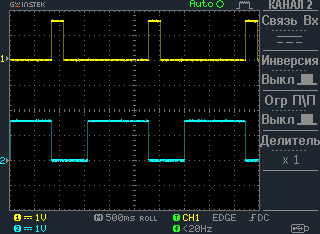
\includegraphics[scale = 1]{img/2_1.png}
	\caption{Осцилограмма обработки прерываний при равных приоритетах обработки прерываний}
\end{figure}

На приведенном рисунке N мы видим, что  время обслуживания запроса прерывания от таймера 2 много больше, чем от таймера 1, но поскольку приоритет прерывания первого таймера не выше второго, то во время обработки прерывания таймера-счетчика 2, прерывание таймера-счетчика 1, хотя и возникает, но не обслуживается.
С целью рассмотрения поведения системы при иных значениях приоритетности добавим в основной цикл файла main.c возможность смены приоритетов во время работы программы.
\lstinputlisting[caption=Код настройки обработки прерываний ,language=c, firstnumber=32, float=h!]{main2_1_2.c}
При подобном подходе, в случае установки более высокого приоритета для обработки прерывания таймера-счетчика 1, последнее будет обработано даже в том случае, если в данный момент не закончилась более длительная по времени обработка прерывания таймера-счетчика 2. 

\begin{figure}[h!]
	\centering
	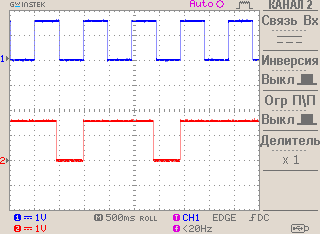
\includegraphics[scale = 1]{img/2_2.png}
	\caption{Осцилограмма обработки прерываний при более высоком приоритете таймера-счетчика 1}
\end{figure}
 

\end{document}